\documentclass[12pt]{article}
\usepackage[utf8]{inputenc}
\usepackage{graphicx} % Allows you to insert figures
\usepackage{subcaption}
\usepackage{amsmath} % Allows you to do equations
\usepackage{fancyhdr} % Formats the header
\usepackage{geometry} % Formats the paper size, orientation, and margins
\usepackage{dirtytalk} % typesetting different types of quotation
\usepackage[english]{babel}
\usepackage{csquotes}
\usepackage{hyperref}
\usepackage{listings}
\lstset{
    language=C,
    basicstyle=\ttfamily, 
    numberstyle=\tiny,
    basicstyle=\small,
    frame=single,
    breaklines=true,
    stepnumber=1,                   % the step between two line-numbers.        
    tabsize=2,                      % sets default tabsize to 2 spaces
    breaklines=true,                % sets automatic line breaking
    breakatwhitespace=true,         % sets if automatic breaks should only happen at whitespace
    title=pseudocode
}

\usepackage{hyperref}

\usepackage{biblatex}
\addbibresource{reffs.bib}

\linespread{1.25} % About 1.5 spacing in Word
\setlength{\parindent}{0.8cm} % No paragraph indents
\setlength{\parskip}{0em} % Paragraphs separated by one line
\renewcommand{\headrulewidth}{0pt} % Removes line in header
\geometry{a4paper, portrait, margin=1in}
\setlength{\headheight}{14.49998pt}

\begin{document}
\begin{titlepage}
   \begin{center}
    \textsc{\large Ministry of Education of Republic of Moldova}\\[0.5cm]
    \textsc{\large Technical University of Moldova}\\[0.5cm]
    \textsc{\large Faculty of Computers, Informatics and Microelectronics}\\[0.5cm]
    \textsc{\large Software Engineering Department}\\[1.2cm]
    
    \vspace{25 mm}
    
    \textsc{\Large Computer Programming}\\[0.5cm]
    \textsc{\large Laboratory work \#3}\\[0.5cm]    % <<<<<<< CHANGE LAB NUMBER HERE
    
    \newcommand{\HRule}{\rule{\linewidth}{0.5mm}}
    \vspace{10 mm}
    \HRule \\[0.4cm]
    { \LARGE \bfseries Two-Dimensional Array Operations and Processing }\\[0.4cm] % <<<<<<< CHANGE LAB TITLE HERE
    \HRule \\[1.5cm]
    
    \vspace{10mm}
    
    \begin{minipage}[t]{0.4\textwidth}
    \begin{flushleft} \large
    \emph{Author:} \\
    Andrei \textsc{Chicu}\\                         % <<<<<<< CHANGE YOUR NAME HERE
    std. gr. FAF-233                                % <<<<<<< CHANGE GROUP NUMBER HERE
    \end{flushleft}
    \end{minipage}
    ~
    \begin{minipage}[t]{0.4\textwidth}
    \begin{flushright} \large
    \emph{Verified:} \\
    Alexandru \textsc{Furdui}\\
    \end{flushright}
    \end{minipage}\\[3cm]
    
    \vspace{5 mm}
    \large Chișinău 2023\\[0.5cm]
    
    \vfill
    \end{center}
\end{titlepage}

\setcounter{page}{2}
\pagestyle{fancy}
\fancyhf{}
\rhead{\thepage}
\lhead{FAF-233 Andrei Chicu; Laboratory Work №3}

% \section*{Introduction}
\section*{Theory Background}
A two-dimensional array is a fundamental data structure used in programming to represent tables, grids, matrices, and other structures with rows and columns. It consists of elements arranged in rows and columns, forming a grid-like structure. Each element in a two-dimensional array is uniquely identified by its row and column indices.

Allocating and freeing memory for a simple (one-dimensional) array is typically easier than doing so for a two-dimensional array because it involves a single continuous block of memory.

In C, a simple array can be treated as a two-dimensional one by mapping the two-dimensional indices (i, j) to a one-dimensional array\\
using the formula \texttt{arr[i * width + j]}\cite{arr_param}. This mapping allows for efficient storage and retrieval of elements in a two-dimensional fashion. By using this formula, one can emulate a 2D array using a 1D array, which can be advantageous in terms of memory efficiency and simplicity of manipulation.

This approach is particularly useful when working with dynamically allocated arrays as allocating and freeing memory for a simple (one-dimensional) array is easier than doing so for a two-dimensional array because it involves a single continuous block of memory.


\section*{The Task}

Describe your task, and enumerate the task/tasks you have implemented:\\
\textbf{Task Hard -- Constructing a Mountain Matrix.}


\section*{Technical implementation}
The full project is here: \url{https://github.com/andyp1xe1/pc_labs/tree/master/lab3}

I defined a structure \texttt{matrix} to represent a 2d array and implemented functions to generate a random matrix, traverse it in a spiral order\cite{spiral}, and sort it using insertion sort. In the main function, I read matrix dimensions, allocated memory, generated and printed a random matrix, sorted it, and printed the sorted result before deallocating memory.
\begin{lstlisting}
# Define a matrix structure
struct Matrix
  int width
  int length
  int[] array
  int[] spiral

# Function to generate random values for the matrix
function generate_matrix(matrix)
  for i from 0 to matrix.length * matrix.width
    matrix.array[i] = random(50, 1000)

# Function to perform a spiral climb on the matrix
function spiral_climb(matrix)
  i_beg = 0
  i_end = 0
  j_beg = 0
  j_end = 0
  i = 0
  j = 0
  k = 0
  while k < matrix.length * matrix.width
    matrix.spiral[k] = i * matrix.width + j
    if i == i_beg and j < matrix.width - j_end - 1
      j = j + 1
    else if j == matrix.width - j_end - 1 and i < matrix.length - i_end - 1
      i = i + 1
    else if i == matrix.length - i_end - 1 and j > j_beg
      j = j - 1
    else
      i = i - 1

    if i == i_beg + 1 and j == j_beg and j_beg != matrix.width - j_end - 1
      i_beg = i_beg + 1
      i_end = i_end + 1
      j_beg = j_beg + 1
      j_end = j_end + 1
    k = k + 1

# Function to swap two integers
function swap(x, y)
  temp = x
  x = y
  y = temp

# Function to sort the matrix using insertion sort on the spiral
function sort_matrix(matrix)
  spiral_climb(matrix)
  for i from 1 to matrix.length * matrix.width
    key = matrix.array[matrix.spiral[i]]
    j = i - 1
    while j >= 0 and matrix.array[matrix.spiral[j]] > key
      matrix.array[matrix.spiral[j + 1]] = matrix.array[matrix.spiral[j]]
      j = j - 1
    matrix.array[matrix.spiral[j + 1]] = key

# Main function
function main()
  matrix m
  print("Input matrix size to be generated and sorted as: len/wid")
  read m.length, m.width
  allocate m.array with size m.length * m.width
  allocate m.spiral with size m.length * m.width
  generate_matrix(m)
  print("Random array:")
  print_matrix(m)
  sort_matrix(m)
  print("Sorted array:")
  print_matrix(m)
  deallocate m.array
  deallocate m.spiral

# Function to print the matrix
function print_matrix(matrix)
  for i from 0 to matrix.length - 1
    for j from 0 to matrix.width - 1
      print(matrix.array[i * matrix.width + j], " ")
    print("\n")
\end{lstlisting}

\pagebreak

\section*{Results}
\hspace{0.8cm}
Describe your results.\\

I have generated a random matrix represented as a unidimensional array.
And have sorted this matrix in a spiral.
\begin{figure}[!h]
  \centering
  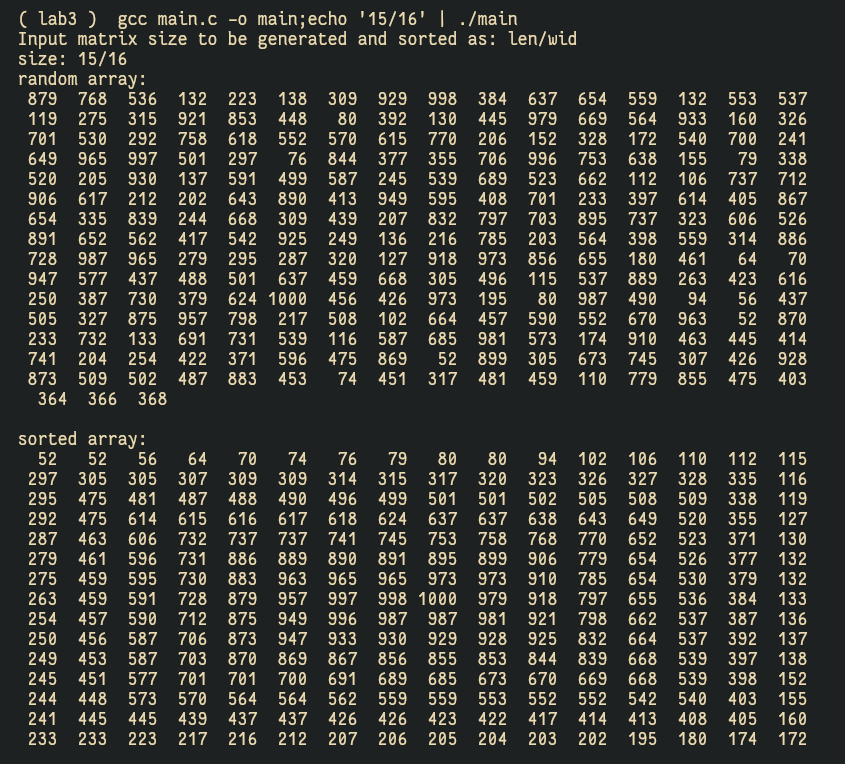
\includegraphics[width=\textwidth]{spiral_matrix.png}
  \caption{spiral matrix}
\end{figure}

\pagebreak

\section*{Conclusion}
In conclusion I can say that working with 2D arrays is much easier when represented as simple arrays, as I can simply pass a pointer to them to a function, and allocating and freeing memory is much more straightforward with a simple array (\texttt{int pointer}).

Also, I have found great value in organising my data with a struct (\texttt{matrix}) as I can simply pass a variable of this type to my various functions instead of repeating myself every time.

This code could be optimised by implementing quick sort, and even maybe using parallel processing to speed up the recursive partitioning.

\pagebreak

\printbibliography

\end{document}
